\documentclass[11pt]{report}

%%%%%%%%%%%%%
%% Imports %%
%%%%%%%%%%%%%
\usepackage[a4paper, margin=2cm, top=2cm, bottom=2cm]{geometry}
\usepackage[utf8]{inputenc}
\usepackage[ngerman]{babel}
\usepackage[usenames, dvipsnames]{xcolor}
\usepackage[framemethod=tikz]{mdframed}
\usepackage{listings}
\usepackage{fancyhdr}
\usepackage[acronyms]{glossaries}
\usepackage{tabularx}
\usepackage{booktabs}
\usepackage{cite}
\usepackage{arydshln}
\usepackage{url}
\usepackage{float}
\usepackage{nameref}
\usepackage{hyperref}

%%%%%%%%%%%%
%% Colors %%
%%%%%%%%%%%%
\definecolor{nordakademie-blue}{RGB}{2,34,94}

%%%%%%%%%%%%%%%%
%% Page Style %%
%%%%%%%%%%%%%%%%
\pagestyle{fancy}
\lhead{\textcolor{nordakademie-blue}{\uppercase{Transferleistung\\ Theorie \& Praxis}}}
\rhead{\textcolor{nordakademie-blue}{
\includegraphics[height=0.85cm,keepaspectratio]{img/NAK-logo}}}
\cfoot{\thepage}
\bibliographystyle{unsrt}
\linespread{1.25}

%%%%%%%%%%%%%%
%% Commands %%
%%%%%%%%%%%%%%
\addto\captionsngerman{\renewcommand{\chaptername}{Abschnitt}}
\newcommand{\inlinecode}{\texttt}
\newcommand*{\SignatureAndDate}[1]{%
    \par\noindent\makebox[2.5in]{\hrulefill}
           \hfill\makebox[2.0in]{\hrulefill}
    \par\noindent\makebox[2.5in][l]{#1}
           \hfill\makebox[2.0in][l]{Datum}
}

%%%%%%%%%%%%%%%%%%%
%% Code listings %%
%%%%%%%%%%%%%%%%%%%
\lstset{% general command to set parameter(s)
  basicstyle=\small, % print whole listing small
  keywordstyle=\color{black}\bfseries\underbar, % underlined bold black keywords
  identifierstyle=, % nothing happens
  commentstyle=\color{white}, % white comments
  stringstyle=\ttfamily, % typewriter type for strings
  showstringspaces=false} % no special string spaces
\lstdefinelanguage{JavaScript}{
keywords={typeof, new, true, false, catch, function, return, null, catch, switch, var, if, in, while, do, else, case, break},
keywordstyle=\color{blue}\bfseries,
ndkeywords={class, export, boolean, throw, implements, import, this},
ndkeywordstyle=\color{darkgray}\bfseries,
identifierstyle=\color{black},
sensitive=false,
comment=[l]{//},
morecomment=[s]{/*}{*/},
commentstyle=\color{purple}\ttfamily,
stringstyle=\color{red}\ttfamily,
morestring=[b]',
morestring=[b]"
}
\lstset{
language=JavaScript,
extendedchars=true,
basicstyle=\footnotesize\ttfamily,
showstringspaces=false,
showspaces=false,
numbers=left,
numberstyle=\footnotesize,
numbersep=9pt,
tabsize=2,
breaklines=true,
showtabs=false,
captionpos=b
}
\renewcommand{\lstlistingname}{Code-Ausschnitt}

%%%%%%%%%%%%%%%%%%%%%%
%% Glossary entries %%
%%%%%%%%%%%%%%%%%%%%%%
\newacronym{bundler}{WAB}{Web Application Bundler}
\newacronym{app}{Web App}{Web Application}
\newacronym{js}{JS}{JavaScript}
\newacronym{html}{HTML}{HyperText Markup Language}
\newacronym{css}{CSS}{Cascading Style Sheets}
\newacronym{cdn}{CDN}{Content delivery network}
\newacronym{hmr}{HMR}{Hot Module Replacement}
\newglossaryentry{cpuTime}
{
  name=CPU-Zeit,
  description={ist die Zeit in welcher ein Prozess Instruktionen auf der CPU ausgeführt hat. Sie unterscheidet sich von der normalen Zeit dahingehend, dass Nutzungen des Prozessors durch andere Prozesse sowie Festplatteninteraktionen nicht mit einfließen\cite{definition:cpuTime}},
  plural=CPU-Zeiten
}
\newglossaryentry{mangling}
{
	name=Name mangling,
	description={Komprimierung von Code durch Umbenennung von Variablen, Funktionen, Klassen und Konstanten}
}
\newglossaryentry{loader}
{
	name=Loader,
	description={Abhängigkeit des Build-Tools, welche dafür zuständig ist, einen bestimmten Dateityp zu verarbeiten}
}
\newglossaryentry{transpilation}
{
	name=Transpilation,
	description={Source zu Source Kompilation}
}
\newglossaryentry{systemTime}
{
	name=Systemzeit,
	description={Die \Gls{cpuTime}, welche im sogenannten Kernel mode verbracht wurde. Um Anweisungen im Kernel mode auszuführen, führt ein Prozess in den häufigsten Fällen die \emph{trap} Instruktion aus, woraufhin in einer Lookup-Table eine Adresse im Kernel-Memory gesucht und ausgeführt wird. Die Systemzeit umfasst Code, welcher in Ring 0 der CPU ausgeführt wird\cite{definition:cpuRings}}
}
\newglossaryentry{userTime}
{
	name=Nutzerzeit,
	description={Die \Gls{cpuTime}, die ein Prozess im isolierten User mode verbringt. Im User mode hat ein Prozess nur Zugriff auf seinen eigenen Speicher und ist dahingehend isoliert, dass er nicht die Stabilität des Systems oder anderer Prozesse beeinträchtigen kann. Die Nutzerzeit umfasst Code, welcher in Ring 3 ausgeführt wird\cite{definition:cpuRings}}
}
\makeglossaries
\makeindex

%%%%%%%%%%%%%%
%% Document %%
%%%%%%%%%%%%%%
\begin{document}

    %%%%%%%%%%%%%%%
    %% Frontpage %%
    %%%%%%%%%%%%%%%
    {\vspace*{0.5cm}\huge Transferleistung 1}
    \vspace{1cm}

    \begin{center}
        \begin{tabularx}{\textwidth}{r|X}
            Matrikelnummer & 8240 \\\midrule
            Thema & Optimierung der Build-Dauer eines Web Application Bundler durch Anpassung der Konfiguration und dessen Auswirkung auf den Entwicklungsprozess \\\midrule
            Studiengang, Zenturie & Angewandte Informatik, A17b\
        \end{tabularx}
    \end{center}
    
    \pagebreak

    \tableofcontents
%    Only useful if there is >3 tables which is not the case in this report
%    \listoftables
%    \listoffigures
    \pagebreak

   	%%%%%%%%%%%%%
    %% Content %%
    %%%%%%%%%%%%%
    \chapter{Einleitung}
    	In der Software-Entwicklung werden häufig Module von anderen Entwicklern in einem Projekt verwendet. Da es in der Webentwicklung im Bereich von \Gls{js}, \Gls{html} und \Gls{css} keinen Buildprozess gibt werden in der klassischen Webentwicklung Abhängigkeiten entweder direkt von sogenannten \Glspl{cdn} eingebunden oder manuell heruntergeladen und in das Projekt kopiert.\\
		Alternativ können Abhängigkeiten per Package-Manager (z. B. \emph{npm\footnote{\url{https://www.npmjs.com}}} oder \emph{yarn\footnote{\url{https://yarnpkg.com/en/}}}) heruntergeladen werden und in einem Bundling-Prozess mit den vorhandenen Modulen des Projektes zu einer Datei kombiniert werden. Dazu werden \Glspl{bundler} wie zum Beispiel \emph{Webpack\footnote{\url{https://webpack.js.org}}} oder \emph{ParcelJS\footnote{\url{https://parceljs.org}}} verwendet.\\
		% TODO Name a source why concatenation of files is useful.
		Zusätzlich zu der Konkatenation von Modulen übernehmen solche Tools die Transformation und \Gls{transpilation} von Eingabedateien, um z. B. Textdateien oder Bilder in den Code zu integrieren, Dateien zu optimieren und komprimieren oder Module, welche in neuen \Gls{js} oder \Gls{css} Versionen geschrieben wurden, in alte Versionen zu übersetzen um Kompatibilität mit älteren Browsern zu gewährleisten.\\
		Intern verwenden diese Tools sogenannte \Gls{loader}, welche einen bestimmten Dateityp verarbeiten und diesen in eine andere Repräsentation bringen. Diese neue Repräsentation kann z. B. ein Bild als Base-64 String in einer JavaScript Datei sein oder die Umwandlung einer Rust-Crate\footnote{Software-Modul, welches in Rust geschrieben wurde, wie z. B. die \href{https://crates.io/crates/stdweb}{stdweb} Crate.} in ein WebAssembly\footnote{https://webassembly.org} Modul.\\
		Die durchschnittliche Aufmerksamkeitsspanne des Menschen beträgt circa zehn Sekunden. Dauert ein Build-Vorgang länger als diese Zeit so besteht die Gefahr, dass der Entwickler sich anderen Aufgaben zuwendet oder die Kaffeetasse auffüllen geht. Entsprechend ist es das Ziel dieser Transferleistung die Builddauer, sofern möglich, auf einen Wert von unter zehn Sekunden zu reduzieren.\\
		\\
		% TODO Name a source of the human attention span
    	Diese Transferleistung befasst sich mit der Beeinflussbarkeit der Build-Zeit eines \Gls{bundler} durch Anpassungen an der Konfiguration in Bezug auf die Geschwindigkeit des Softwareenwicklungsprozess. In dieser Arbeit werden die folgenden Forschungsfragen näher beleuchtet:
	    	\begin{enumerate}
		    	\item Ist die Build Performance relevant für den Entwicklungsprozess? \label{question0}
		    	\item Welche Faktoren haben eine Auswirkung auf die Dauer des Build? \label{question1}
		    	\item Lassen sich diese Faktoren in einem Software-Projekt beeinflussen? \label{question2}
		    \end{enumerate}

		\section{Bezug zu der PPI AG}
			Bei der PPI AG gibt es mehrere Software-Entwicklungsprojekte, die unter anderem die Entwicklung einer Web-App umfassen. Dies schließt zum Beispiel das Studenten-Verwaltungstool \emph{StuMaTo} ein, welches der Verwaltung und Verteilung von Aufgaben für Studenten dient. Dieses Tool wird durch ein kleines Team von Studenten weiterentwickelt werden, wobei eine direkte Relevanz der Ergebnisse dieser Transferleistung sich positiv auf den Entwicklungsprozess auswirken könnte, da ein \Gls{bundler} eingesetzt wird.

	\chapter{Methodik}
		\label{section:method}
		Um die Forschungsfrage \ref{question1} zu beantworten ist ein Projekt nötig, an dem empirisch untersucht werden kann, welche Faktoren einen Einfluss auf die Build-Zeit haben. Da bei der PPI AG aktuell kein Software-Projekt existiert, welches ein \Gls{bundler} im Einsatz hat und Boilerplates sowie Beispielprojekte aus dem Internet potentiell unbedachte Nebeneffekte hervorrufen können, wird im Rahmen dieser Transferleistung eine rudimentäre \Gls{app} aufgesetzt. Diese wird sich vom Umfang auf die für den Build Prozess relevanten Kriterien beschränken um eine Analyse der Faktoren, welche die Build Zeit beeinflussen, zu ermöglichen.
		\section{Beispielprojekt}
			Im Folgenden werden die einzelnen Komponenten für das Beispielprojekt beschrieben und die Auswahl begründet.
			\paragraph{\Gls{bundler}} Um die Anwendbarkeit der Ergebnisse zu maximieren, wurde für dieses Projekt der am weitesten verbreitete \Gls{bundler} \emph{Webpack}\cite{npmtrends:wab} verwendet, um eine möglichst einfache Übertragung der Konfigurationsoptionen auf andere Projekte zu ermöglichen. Dies bietet zusätzlich den Vorteil von einer großen Informationsvielfalt bezüglich der Konfiguration.

			\paragraph{React} Bei der Entwicklung von \Glspl{app} werden häufig Frameworks wie z. B. React\footnote{\url{https://reactjs.org}}, Angular\footnote{\url{https://angular.io}} oder VueJS\footnote{\url{http://vuejs.org}} verwendet. In diesem Projekt wurde \emph{React} aufgrund seiner Popularität\cite{npmtrends:frameworks} und den vorhandenen Kenntnissen des Autors verwendet.

			\paragraph{Material UI} Als Library für grafische Komponenten wurde das Projekt \emph{Material UI}\cite{frameworks:material-ui} gewählt, da es aufgrund der vorhandenen Beispiele in der Dokumentation ein schnelles Prototyping der Dummy-UI ermöglicht. Außerdem wurde die Schriftart Roboto\footnote{\url{https://fonts.google.com/specimen/Roboto}} und das Material-UI Icon-Set\footnote{\url{https://www.material.io/tools/icons/?style=baseline}} von Google eingebunden, da sie den UI Guidelines\cite{guidelines:material-ui} der Library entsprechen und von dieser empfohlen werden.

			\paragraph{Victory Graphs} Um den Umfang des Projektes zu erweitern und ein möglichst realistisches Szenario für die Build-Zeit zu erreichen wurde zusätzlich eine Abhängigkeit für Diagramme eingebunden. Hierbei wurde \emph{Victory}\cite{frameworks:victory} gewählt, da es eine einfache und gut dokumentierte Integration mit React bietet.

		\section{Messverfahren}
			Um eventuelle Ungenauigkeiten durch Unterschiede in der Prozessorauslastung oder eventuelle Caches zu minimieren wird der Build mehrfach ausgeführt und die durchschnittliche Dauer berechnet. Dabei geht der erste Build nach Anpassung der Konfigurationsdatei nicht mit in die Wertung ein, da er mögliche Abweichungen durch Caching aufweisen könnte. Um ein realistisches Szenario zu schaffen, werden anschließend für jeden Datenpunkt jeweils zwei Builds ausgeführt. Der erste Build wird dabei mit der Ausgangslage des Projekt durchgeführt. Im Anschluss wird der Inhalt einer Datei verändert und ein weiterer Vorgang gestartet. Die \Gls{cpuTime}, die dieser zweite Build benötigt, wird gemessen und in die Wertung aufgenommen. Das Messverfahren wurde durch ein Python-Script automatisiert, welches auf \href{https://github.com/TexNAK/WebBundlerOptimization/blob/40c8c00dee7af6970bc82c29e2fc0f3cfd6c12eb/webpack-project/runBuilds.py}{GitHub} zu finden ist. Zusätzlich zu der \Gls{cpuTime} nimmt das Script ein Speicherprofil auf, welches im Folgenden genutzt wird um Optimierungen in der Speichernutzung zu finden\footnote{Da ein zu hoher Speicherverbrauch auf Geräten mit geringem Arbeitsspeicher zu Swapping und somit Performanceverlusten führen kann, wird dieses mit beleuchtet.}.\\
			Da Abbildung \ref{figure:baseline_duration} zeigt, dass es nur minimale Abweichungen von bis zu $\pm 3 \%$ zwischen den einzelnen Datenpunkten gibt, werden im Folgenden zehn Datenpunkte erfasst und der Durchschnitt gebildet.
				% TODO Maybe a source why Swapping is slow
			
			\paragraph{Leistungsmerkmale des Rechners} Sämtliche Builds werden auf einem Retina MacBook aus dem Jahr 2017 mit 8 GB RAM und einem Intel Core i7 mit macOS 10.14 durchgeführt. Während des Build werden sämtliche Anwendungen, welche nicht für die Ausführung des Betriebssystems oder des Builds kritisch sind, geschlossen um eine möglichst reproduzierbare Umgebung zu schaffen. Es wird dabei darauf geachtet, dass das Gerät während der Messungen an eine Stromquelle angeschlossen und ausreichend gekühlt ist, um CPU throttling zu vermeiden.

		\section{Gruppierung der Anpassungen}
			Die Analyse der möglichen Optimierungen wird in mehreren Schritten durchgeführt.
			\paragraph{Grundlage}\label{baseline-build} Zu Beginn wird das Beispielprojekt mit einer Konfiguration\footnote{Die vollständige Konfigurationsdatei ist im Anhang auf Seite \pageref{baseline-build} zu finden.} gebaut, die einer typischen Produktionsumgebung ähnelt. Die resultierende Builddauer wird als Grundlage für den Vergleich mit potenziellen Optimierungen genommen, welchen in den folgenden Schritten durchgeführt werden.
				% TODO Add a source for the "typical" production config

			\paragraph{Umgebungsunabhängig} Im zweiten Schritt werden verschiedene Aspekte der Konfigurationsdatei angepasst, welche keine signifikanten Auswirkungen auf die resultierenden Build-Artefakte haben\footnote{Die Größe der Ausgabedatei darf um nicht mehr als $5 \%$ abweichen und die Browser-Kompatibilität sowie Funktionalität nicht beeinträchtigt werden.}, und ihre individuellen Auswirkungen unabhängig voneinander gemessen.

			\paragraph{Destruktive Anpassungen} Einige Änderungen haben negative Auswirkungen auf die resultierenden Build-Artefakte, wie zum Beispiel eine größere Ausgabedatei oder verminderte Browser-Kompatibilität\footnote{JavaScript ist zwar ein Standard aber viele der Funktionen der Sprache werden nur von einem Teil der Browser und deren Versionen unterstützt. Ein Überblick über die verfügbaren Versionen pro Browser und dessen Version kann auf \href{https://caniuse.com/}{caniuse.com} gefunden werden.}. Im dritten Schritt werden Anpassungen vorgenommen, welche solch negativen Auswirkungen haben. Diese werden wie zuvor unabhängig voneinander gemessen.

			\paragraph{Gesamtbewertung} Im letzten Schritt werden sämtliche Änderungen gemeinsam angewendet. Dies wird zunächst für die umgebungsunabhängigen Anpassungen und anschließend für alle durchgeführt. Dies dient dazu, eventuelle Interaktionen zwischen Konfigurationsänderungen abzudecken und einen Gesamtwert für die Verbesserung in der Build-Zeit zu erhalten.
	\clearpage

	\chapter{Evaluation}
		Im Folgenden wird die in Abschnitt \ref{section:method} beschriebe Methodik angewendet. Die gewählten Optimierungen wurden auf Basis ihrer Komplexität und der erwarteten Verbesserung ausgewählt. Bis auf Abschnitt \ref{section:minification} sind alle Anpassungen an der Konfiguration durch die Dokumentations-Website von Webpack inspiriert worden\cite{optimization-source:webpack}.
	
		\section{Ausgangslage}
			Wie auf Seite \pageref{baseline-build} erwähnt wurde zunächst eine Basismessung durchgeführt. Die genutzte Konfigurationsdatei kann im Anhang auf Seite \pageref{figure:baselineConfiguration} oder auf \href{https://github.com/TexNAK/WebBundlerOptimization/blob/d018b3e0db6a861c4f41e38e7265ca8f9d500319/webpack-project/webpack.config.js}{GitHub} gefunden werden.			\paragraph{Abbildung \ref{figure:baseline_duration}} zeigt die \Gls{cpuTime} der einzelnen Ausführungen. Auf der x-Achse sind die einzelnen Läufe verteilt. Die y-Achse stellt die gemessene Zeit dar, welche in \Gls{systemTime} und \Gls{userTime} geteilt ist. Die Abbildung zeigt eine durchschnittliche Zeit von $26$ Sekunden mit einer maximalen Abweichung von $3 \%$. Aufgrund der geringen Abweichung in Verteilung und Gesamtdauer wird in den nachfolgenden Messungen nur die durchschnittliche Dauer betrachtet. Da die Messungen nur alle $0,25$ Sekunden stattfinden wird die Dauer auf die nächste natürliche Zahl gerundet.
			\paragraph{Abbildung \ref{figure:baseline_memory}} zeigt den Speicherverbrauch des \Gls{bundler}, wobei die x-Achse die vergangene Zeit seit Prozessstart und die y-Achse den Speicherverbrauch in Megabyte darstellt. Auch bei diesem Graph ist nur eine geringe Abweichung vom Durchschnitt zwischen den einzelnen Durchgängen sichtbar. Da die internen Vorgänge des \Gls{bundler} nicht genauer bekannt sind und daher die Speicherkurve nicht weiter erläutert werden kann, wird im Folgenden nur der maximale Speicherverbrauch betrachtet.

			\begin{figure}[p]
	            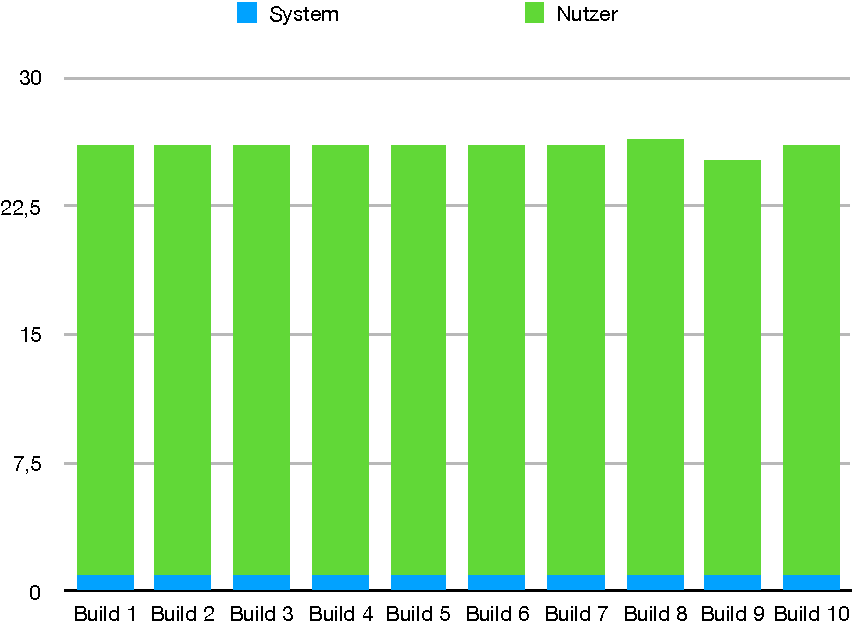
\includegraphics[width=\textwidth]{img/baseline_duration.pdf}
	            \caption{Basismessung | CPU Zeit}
	            \label{figure:baseline_duration}
	        \end{figure}
	        \begin{figure}[p]
	            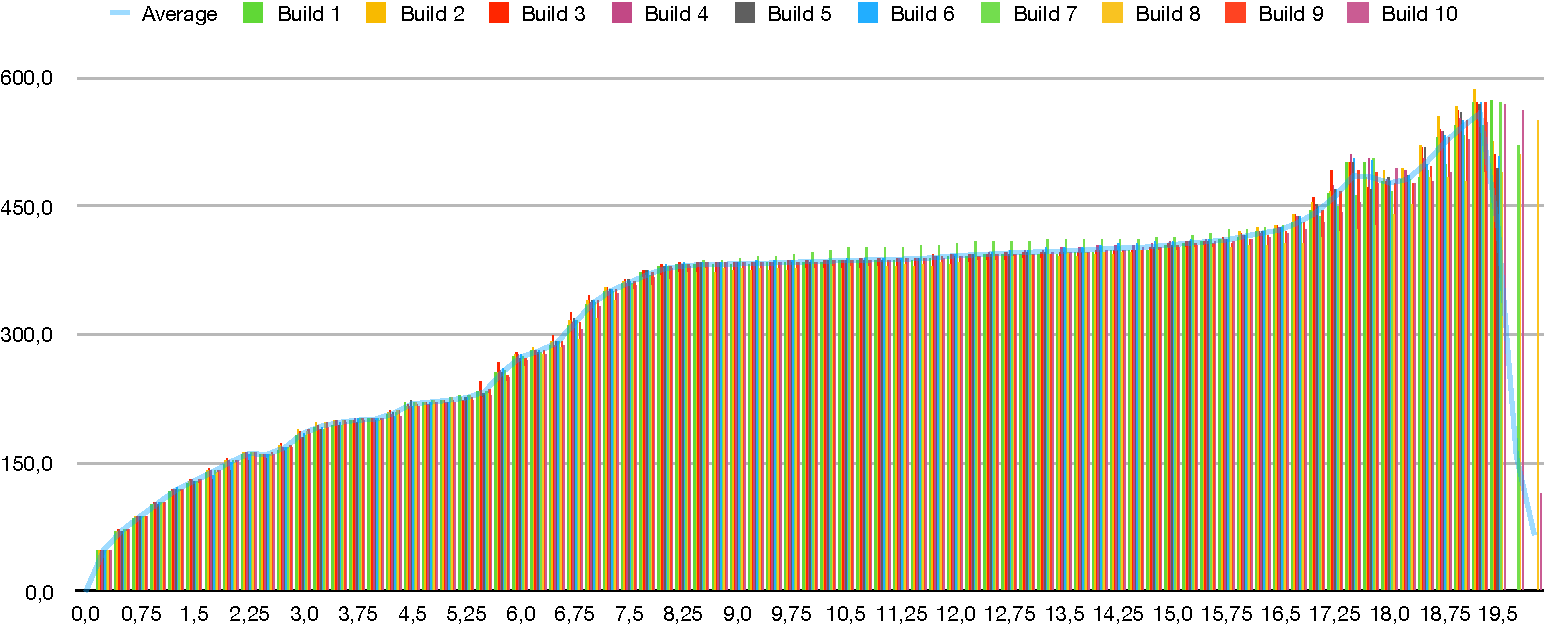
\includegraphics[width=\textwidth]{img/baseline_memory.pdf}
	            \caption{Basismessung | Speicherverbrauch}
	            \label{figure:baseline_memory}
	        \end{figure}

        \section{Nicht destruktive Anpassungen}
        	\label{section:productionOptimizations}
        	\subsection{Optimierung der Minifikation}
        		\label{section:minification}
	        	Das Ersetzen von Leerzeichen und Zeilenumbrüchen bringt die meiste Platzersparnis in kurzer Zeit. Das Umstrukturieren und Optimieren von Code ist hingegen zeitaufwändig und bringt vergleichsweise geringe Verbesserungen\cite{optimization-source:minify}.
        		\subsubsection{Ohne Codeoptimierung}
        			\label{section:minification_noCompress}
	        		Durch das Deaktivieren der Code-Optimierung wurde die \Gls{cpuTime} um \emph{12,64} Sekunden auf \emph{13} Sekunden reduziert. Die Größe der Ausgabedatei hat sich dabei nur um $+2$ Kilobyte auf insgesamt $932$ kB vergrößert.\\
	        		Der maximale Speicherverbrauch lag im Durchschnitt bei $369$ MB.\\
		        	Um die Optimierung zu deaktivieren, muss in der Konfigurationsdatei Zeile 97 durch folgende ersetzt werden:\\
		        	\begin{center}
			        	\lstset{%
						    caption=Deaktivierung der Codeoptimierung,
							basicstyle=\footnotesize,
							xleftmargin=.2\textwidth,
							xrightmargin=.2\textwidth,
							numbers=none
						}
			        	\begin{lstlisting}[language=JavaScript]
							uglifyOptions: {
								compress: false
							}
			        	\end{lstlisting}
		        	\end{center}
		        	Die vollständige Konfigurationsdatei kann auf \href{https://github.com/TexNAK/WebBundlerOptimization/compare/master...nondestr_scopedCompilation#diff-1fb5683b1e7adbcee273b7f9f9a08a22}{GitHub} eingesehen werden.
		        	
%			        \begin{figure}[p]
%			            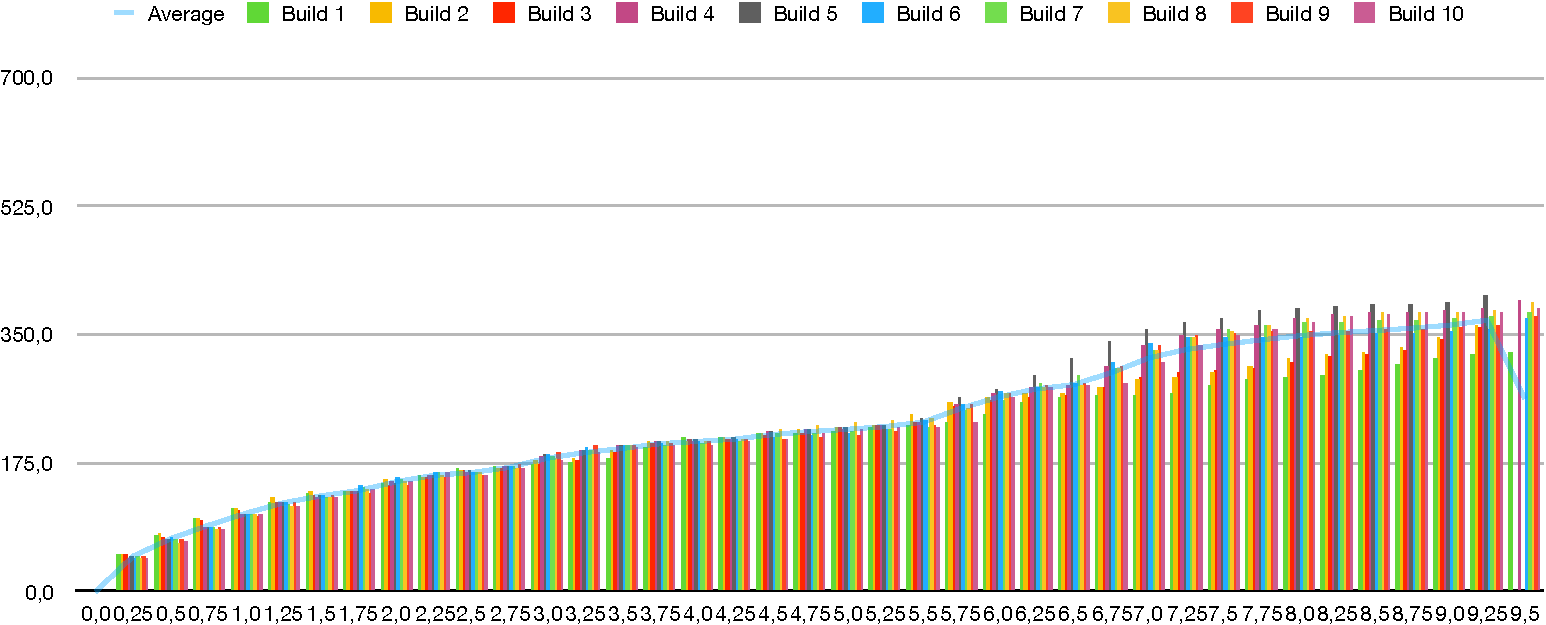
\includegraphics[width=\textwidth]{img/nondestr_minify_nocompress_memory}
%			            \caption{Minifikation (compress=false) | Speicherverbrauch}
%			            \label{figure:minification_noCompress_memory}
%			        \end{figure}

        		\subsubsection{Ohne Mangling}
	        		Durch das Deaktivieren des \Gls{mangling} wurde die \Gls{cpuTime} um \emph{3} Sekunden auf \emph{23,34} Sekunden reduziert. Die Größe der Ausgabedatei hat sich dabei um weniger als $1$ kB verändert.\\
	        		Der maximale Speicherverbrauch lag im Durchschnitt bei $395$ MB.\\
        			Die Konfigurationsdatei ist großteils identisch mit der in Sektion \ref{section:minification_noCompress} gezeigten mit dem Unterschied, dass statt der Option \emph{compress} die Option \emph{mangle} auf \emph{false} gesetzt wurde.
        			
%			        \begin{figure}[p]
%			            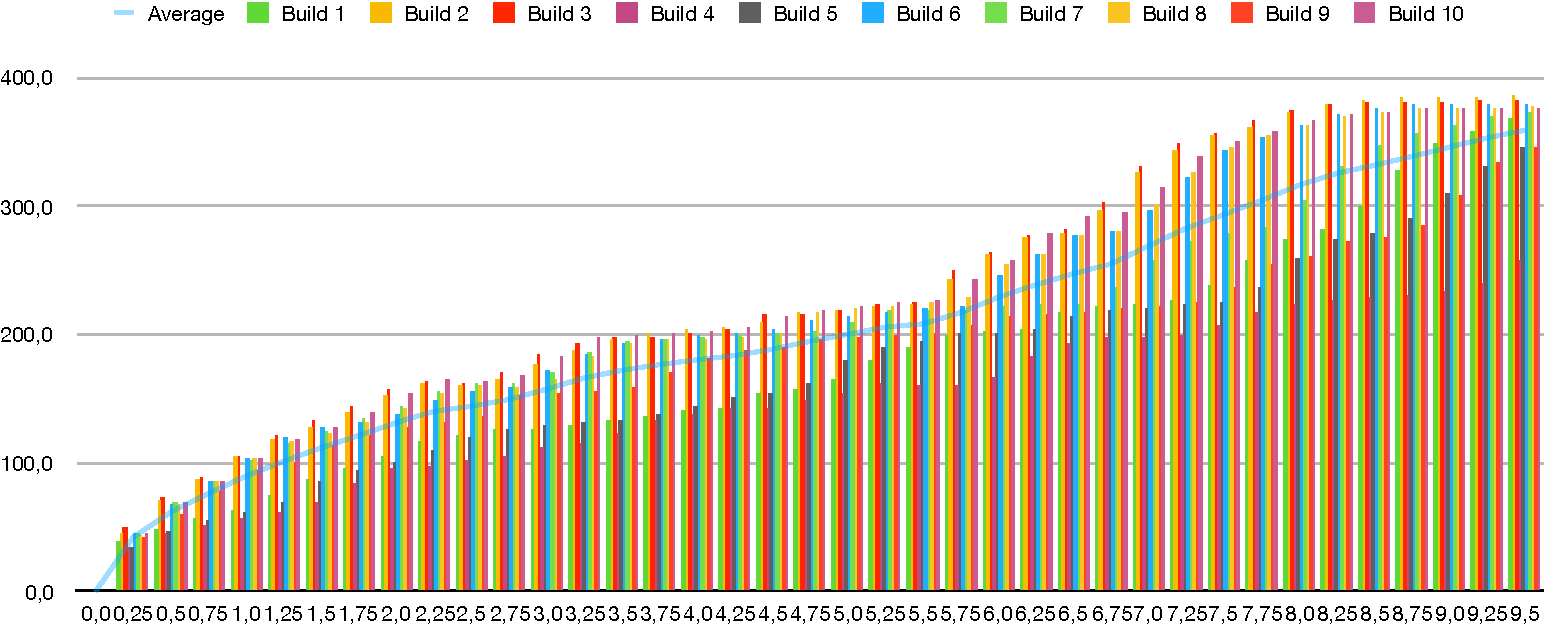
\includegraphics[width=\textwidth]{img/nondestr_minify_nomangle_memory}
%			            \caption{Minifikation (mangle=false) | Speicherverbrauch}
%			            \label{figure:minification_noMangle_memory}
%			        \end{figure}

        	\subsection{Scoped compilation}
        		\label{section:scopedCompilation}
        		Es ist möglich einen Teil der Abhängigkeiten und auch Teile des Projektes, welche sich nur selten ändern, einmalig zu bauen und in nachfolgenden Builds lediglich einzubinden. Da die meisten Projekte zu einem Großteil aus Abhängigkeiten bestehen\footnote{Ein mit create-react-app v1.5.2 erstelltes Projekt hat 967 Dependencies mit ca. 13.000 JS-Dateien} kann dies zu signifikanten Zeitersparnissen führen.\\
        		Um Scoped compilation zu nutzen, muss eine neue Konfiguration erstellt werden, die den extra Build beschreibt. Die genutzte Konfiguration ist im Anhang auf Seite \pageref{vendorConfig} zu finden. Sie beinhaltet die sechs größten Abhängigkeiten des Projektes. Zusätzlich muss in der normalen Konfiguration die Ausgabedatei des externen Build geladen werden. Dazu muss der folgende Code zwischen Zeile 79 und 90 eingefügt werden:\\
        		\begin{center}
		        	\lstset{%
					    caption=Einbindung der Scoped compilation,
						basicstyle=\footnotesize,
						numbers=none
					}
		        	\begin{lstlisting}[language=JavaScript]
						new webpack.DllReferencePlugin({
		            context: process.cwd(),
		            manifest: require(path.join(outputPath, 'ReactStuff.json'))
		        }),
		        	\end{lstlisting}
	        	\end{center}
        		
        		Durch diese Auslagerung wurde die \Gls{cpuTime} des Build dadurch auf \emph{3} Sekunden reduziert, was eine Beschleunigung um den Faktor \emph{8,7} gegenüber der Ausgangslage darstellt. Da die größten Abhängigkeiten ausgelagert sind hängt die Dauer des Builds nun lediglich von den eigentlichen Projektdateien ab. Die sehr geringe Zeit lässt sich auf die geringe Größe des Beispielprojektes zurückführen. Die reale Zeitersparnis hängt somit direkt von der Menge der Abhängigkeiten und Modulen des Projektes ab, welche man in einen extra Build auslagert.\\
        		Ein weiterer Aspekt ist, dass der Speicherverbrauch des Buildprozesses ebenfalls signifikant von maximal $550$ MB auf $150$ MB gesenkt wurde. Auf Geräten mit geringem Arbeitsspeicher kann dies von Relevanz sein um Swapping und die damit einhergehenden Performanceverluste zu vermeiden.\\
        		Die Konfigurationsdatei für den Build kann auf \href{https://github.com/TexNAK/WebBundlerOptimization/compare/master...nondestr_scopedCompilation#diff-1fb5683b1e7adbcee273b7f9f9a08a22}{GitHub} eingesehen werden.

%				\begin{figure}[p]
%		            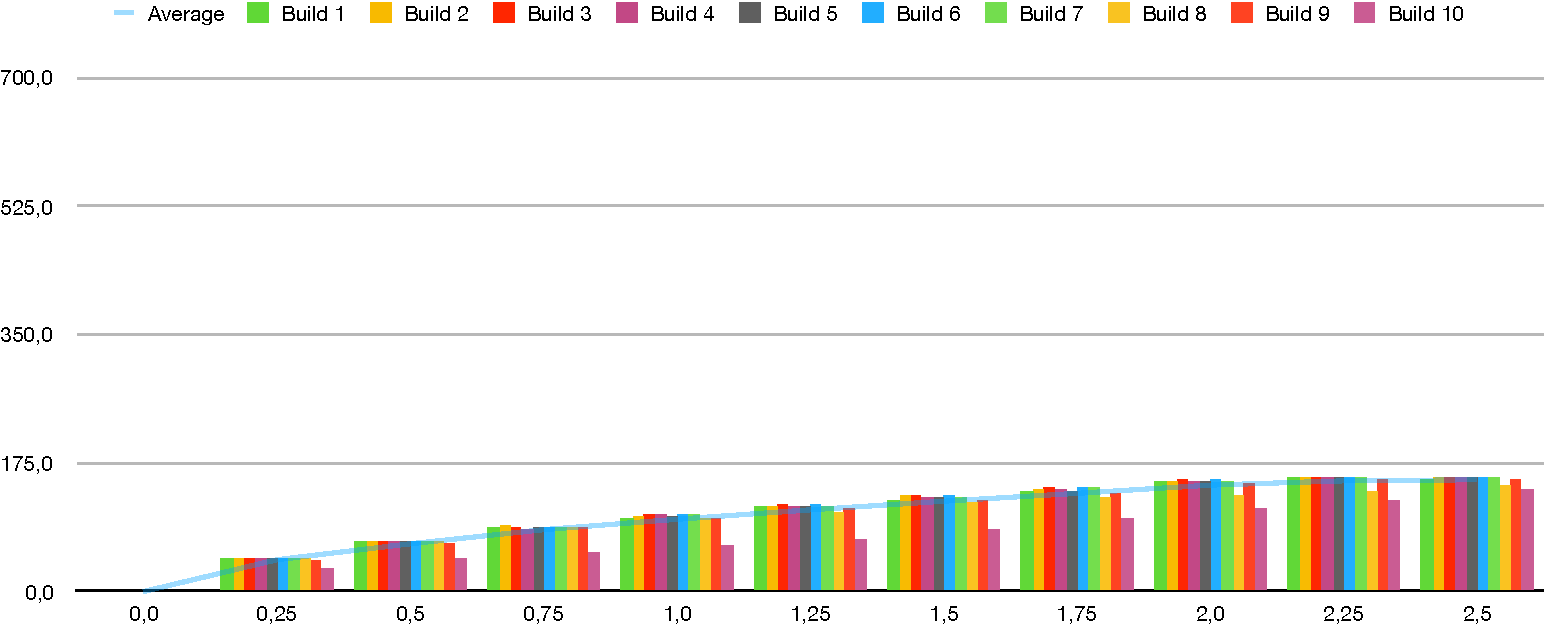
\includegraphics[width=\textwidth]{img/nondestr_scopedCompilation_memory}
%		            \caption{Scoped compilation | Speicherverbrauch}
%		            \label{figure:scopedCompilation_memory}
%		        \end{figure}

    		\subsection{Caching}
    			Es besteht die Möglichkeit die Ausgaben ausgewählter \Gls{loader} zu cachen. In dem Beispielprojekt macht der \emph{babel-loader} mit ca. \emph{4} Sekunden einen Großteil der Zeit aus, welche von Loadern in Anspruch genommen wird. Daher wurde dieser gecached. Als Resultat wurde die \Gls{cpuTime} auf \emph{23} Sekunden reduziert. Der maximale Speicherverbrauch lag im Durchschnitt bei $442$ MB.\\
    			Um Caching zu aktivieren, muss der Code in der Konfiguration von Zeile 53 bis 61 ersetzt werden durch den folgenden:
    			\begin{center}
		        	\lstset{%
					    caption=Caching,
						basicstyle=\footnotesize,
						xleftmargin=.15\textwidth,
						xrightmargin=.15\textwidth,
						numbers=none
					}
		        	\begin{lstlisting}[language=JavaScript]
				use: ['cache-loader', {
				    loader: 'babel-loader',
				    options: {
				        compact: true,
				        cacheDirectory: true,
				        plugins: ['transform-class-properties'],
				        presets: ['env', 'react']
				    }
				}]
		        	\end{lstlisting}
	        	\end{center}
    			Die vollständige Konfiguration kann auf \href{https://github.com/TexNAK/WebBundlerOptimization/commit/370e3233461f32c823e6c794ad52179e15391ebc#diff-1fb5683b1e7adbcee273b7f9f9a08a22}{GitHub} eingesehen werden.
    			
%    			\begin{figure}[p]
%		            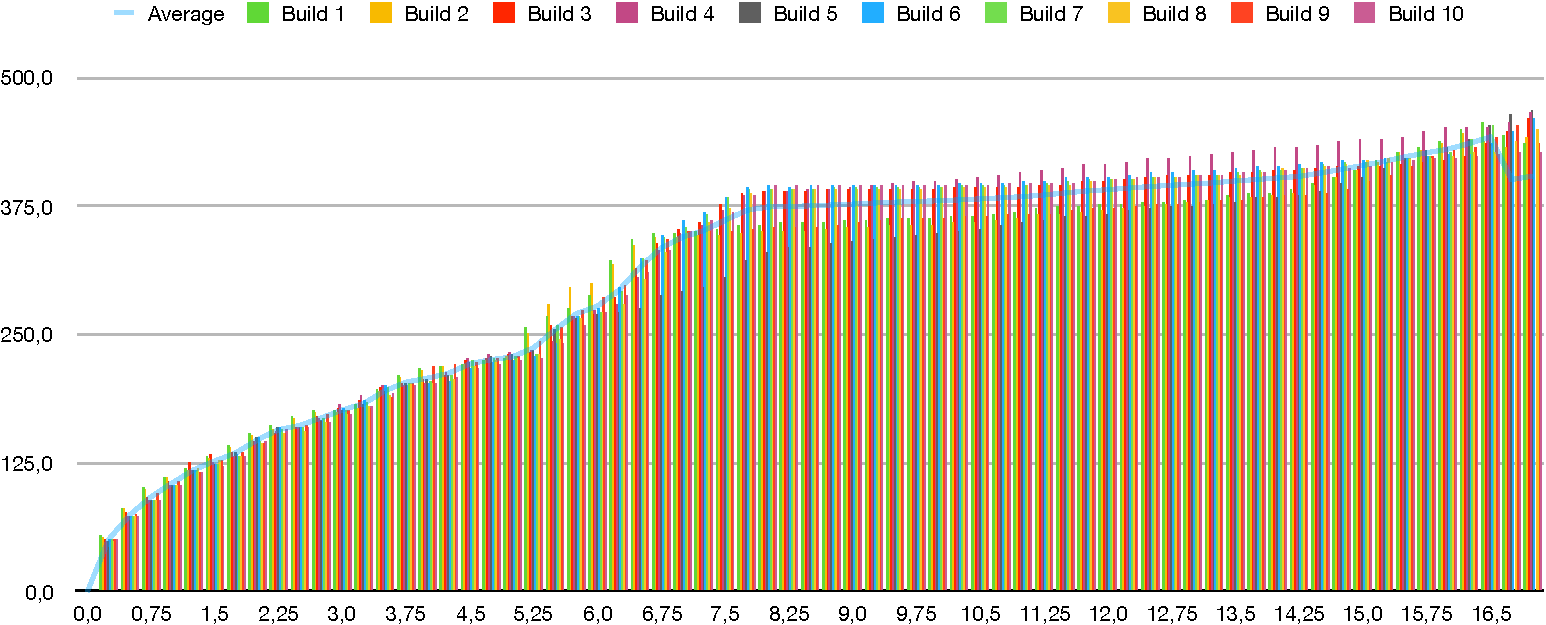
\includegraphics[width=\textwidth]{img/nondestr_cache_memory}
%		            \caption{Cache | Speicherverbrauch}
%		            \label{figure:cache_memory}
%		        \end{figure}

    	\section{Destruktive Anpassungen}
    		\subsection{Source-Maps}
    			Um den Code nach dem Buildprozess noch debuggen zu können und Stack-Traces für Exceptions mit den entsprechenden Source-Dateien zu verbinden wird eine sogenannte Source-Map gebaut, welche die Relation zwischen den Zeilen in der Ausgabedatei und der Eingabedatei beinhalten. Im Normalfall werden diese Source-Maps für alle Dateien auf Zeilenbasis erzeugt. Es gibt die Möglichkeit die Source-Maps nur auf Datei-/Modulbasis zu erzeugen. Eine Umstellung auf die modulbasierte Erzeugung resultierte in einer \Gls{cpuTime} von \emph{12} Sekunden. Sofern Source-Maps für die Entwicklung nicht benötigt werden, können diese auch komplett deaktiviert werden.\\
    			Es gab keine signifikanten Abweichungen im Speicherverbrauch in Relation zur Ausgangslage.\\
    			Um Source-Maps auf Modulbasis zu erzeugen, muss Zeile 11 der Konfigurationsdatei zu dem folgenden geändert werden:
    			\begin{center}
		        	\lstset{%
					    caption=Caching,
						basicstyle=\footnotesize,
						xleftmargin=.15\textwidth,
						xrightmargin=.15\textwidth,
						numbers=none
					}
		        	\begin{lstlisting}[language=JavaScript]
		        		devtool: 'cheap-module-eval-source-map',
		        	\end{lstlisting}
	        	\end{center}  
    			Die vollständige Konfiguration kann auf \href{https://github.com/TexNAK/WebBundlerOptimization/compare/master...destr_cheapSourceMaps#diff-1fb5683b1e7adbcee273b7f9f9a08a22}{GitHub} eingesehen werden.

%				\begin{figure}[p]
%		            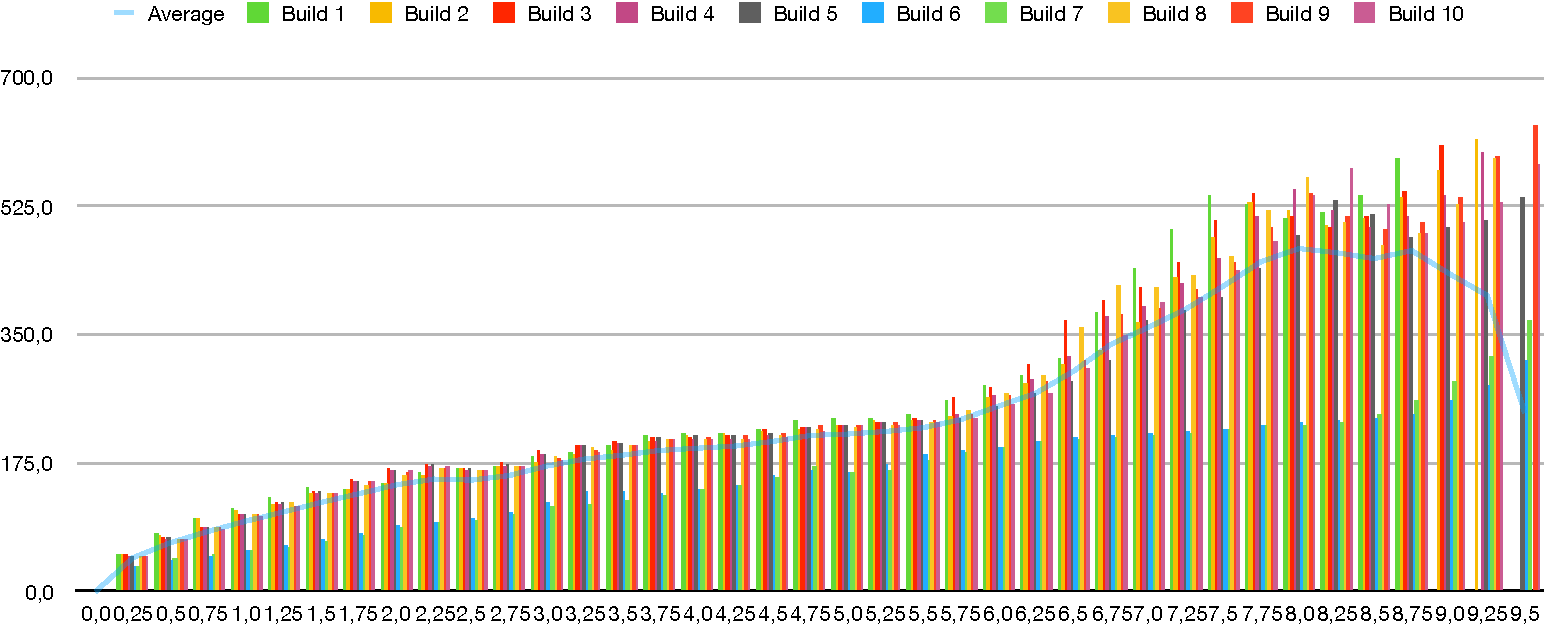
\includegraphics[width=\textwidth]{img/destr_sourceMaps_cheap_memory}
%		            \caption{Source Maps (modulbasiert) | Speicherverbrauch}
%		            \label{figure:sourceMaps_memory}
%		        \end{figure}

    		\subsection{Inkrementelle Builds \& In-Memory-Kompilation}
    			\label{section:incrementalBuilds}
    			Normalerweise werden die Ausgabedateien auf die Festplatte geschrieben und bei jedem Build vollständig neu durchgeführt. Es besteht die Möglichkeit die Ausgabedateien im Speicher zu halten und davon ausgehend inkrementelle Builds durchzuführen. Im Fall des Beispielprojektes wurde dadurch die \Gls{cpuTime} auf \emph{30} Sekunden angehoben. Dabei ist zu beachten, dass die \Gls{cpuTime} bei diesen Messungen nicht nur den reinen Build, sondern auch die zusätzliche Speicherverwaltung sowie File-Watcher o.ä. beinhaltet. Außerdem konnte die \Gls{cpuTime} nicht wie in den vorherigen Fällen automatisch gemessen werden, sondern wurde manuell dem macOS Activity-Monitor entnommen. Dabei wurde der Server gestartet und gewartet, bis die \Gls{cpuTime} sich über einen Zeitraum von zehn Sekunden nicht mehr verändert. Anschließend wurde eine Datei angepasst, wodurch ein neuer Build gestartet wird. Es wurde erneut wie oben vorgegangen, um die \Gls{cpuTime} zu entnehmen. Die Differenz der beiden Zeiten wurde als Datenpunkt aufgenommen. Dieses Vorgehen wurde für zehn Werte wiederholt und der Durchschnitt gebildet. Um inkrementelle Builds zu nutzen, sind keine Anpassungen an der Konfiguration nötig. Es muss statt dem Befehl \emph{webpack} der Befehl \emph{webpack-dev-server} ausgeführt werden, welcher zuvor installiert werden muss\footnote{\url{https://github.com/webpack/webpack-dev-server}}.

    		\subsection{\Gls{hmr}}
    			Ein weiteres Feature ist das sogenannte \Gls{hmr}. Dies ermöglicht es einen Teil des Projektes neu zu bauen und das alte Modul in einer offenen Instanz der Seite durch das neue zu ersetzen. Dieses Feature setzt jedoch die in Sektion \ref{section:incrementalBuilds} beschriebene In-Memory-Kompilation voraus. Im Durchschnitt nahm der Build \emph{35} Sekunden \Gls{cpuTime} in Anspruch.\\
    			Um \Gls{hmr} zu aktivieren, müssen die Anweisungen aus Abschnitt \ref{section:incrementalBuilds} befolgt und zusätzlich die folgenden Anpassungen angewendet werden:\\
    			\begin{center}
		        	\lstset{%
					    caption=\Gls{hmr},
						basicstyle=\footnotesize,
						numbers=none
					}
		        	\begin{lstlisting}[language=JavaScript]
			/* Zeile 12 */ devServer: { hot: true, contentBase: './dist' },
			/* Zeile 58 */ plugins: ['react-hot-loader/babel', 'transform-class-properties'],
			/* Zeile 59 */ presets: ['env', 'react', 'react-hmre'],
			/* Zeile 99 */ new webpack.HotModuleReplacementPlugin()
		        	\end{lstlisting}
	        	\end{center}
    			Die vollständige Konfigurationsdatei kann auf \href{https://github.com/TexNAK/WebBundlerOptimization/commit/4a1cadbe86cc305bafeb9f7d56733fc90b0f514a#diff-1fb5683b1e7adbcee273b7f9f9a08a22}{GitHub} eingesehen werden.

		\section{Gesamtbewertung}
			\subsection{Umgebungsunabhängig}
				Wenn man sämtliche in Abschnitt \ref{section:productionOptimizations} beschriebenen Optimierungen in einer Konfiguration gemeinsam anwendet, so erreicht man bei dem Beispielprojekt eine \Gls{cpuTime} von \emph{2} Sekunden. Da diese Zeit sehr nah an der Zeit der durch Scoped Compilation alleine erreichten Zeit liegt, ist zu vermuten, dass die anderen beschriebenen Optimierungen hauptsächlich die Abhängigkeiten betroffen haben, welche durch Scoped Compilation aus dem Build extrahiert wurden.
			\subsection{Gesamtmessung}
				Fügt man alle Anpassungen zusammen so erreicht man eine durchschnittliche Build-Zeit von insgesamt \emph{3} Sekunden. Da der Build nun aber In-Memory durchgeführt wird, führt der \emph{cache-loader} zu zusätzlichem Overhead, da die Zwischenschritte des Builds auf der Festplatte gespeichert werden. Entfernt man diesen aus der Konfiguration, so erreicht man eine Zeit von \emph{1} Sekunden.
				
		\section{Relevanz der Builddauer}
			In den meisten Programmiersprachen gibt es einen Buildprozess. Ziel dieses Vorgangs ist es, den Code in eine ausführbare Form zu übersetzen. Im Fall von Sprachen wie z. B. C++, Swift oder Rust ist diese Form die Maschinensprache. Bei Java oder Scalar ist es der Java Bytecode und bei Sprachen wie TypeScript, CoffeeScript oder JavaScript\footnote{Bei JavaScript wird der Code zwischen JavaScript Versionen transpiliert um Rückwärts-Kompatibilität zu gewährleisten.} ist es JavaScript. In jedem Fall kann man davon ausgehen, dass zum Testen und Ausführen des Codes ein solcher Build durchlaufen werden muss. Wenn kleine Anpassungen am Source-Code (z. B. die Änderung einer Farbe) durchgeführt werden und die Resultate geprüft werden sollen, so ist es von Vorteil, wenn der Vorgang eine möglichst kurze Zeit in Anspruch nimmt, um den Entwicklungsprozess zu beschleunigen. Folglich ist die Antwort auf die Forschungsfrage \ref{question0}, dass die Performance eine Relevanz in dem Entwicklungsprozess hat.

	\chapter{Auswertung}
		In Tabelle \ref{table:optimizationResultOverview} sind sämtliche Messergebnisse noch einmal mit der \Gls{cpuTime} und dem maximalen Speicherverbrauch aufgeführt. Der zweite Block beinhaltet alle umgebungsunabhängigen (nicht destruktiven) Anpassungen, der dritte die destruktiven Anpassungen und der letzte Block die Gesamtwerte. Betrachtet man alle Optimierungen so hat die \nameref{section:scopedCompilation} die größten Einsparung zur Folge gehabt. Kombiniert ergeben die Optimierungen der Minifikation die zweitbeste Optimierung und modulbasierten Source-Maps resultieren in einem nahezu identischen Resultat. Eine grafische Übersicht der Optimierungen ist in Abbildung \ref{figure:resultGraph} zu finden. Caching, Inkrementelle In-Memory Builds sowie \Gls{hmr} haben dabei nur minimale Verbesserungen bzw. teils sogar Verschlechterungen der Build-Zeit zur Folge gehabt. Dabei ist allerdings zu betrachten, dass \Gls{hmr} selbst einen großen Vorteil im Entwicklungsprozess bietet. Durch das Updaten von einzelnen Modulen in einer laufenden Instanz der Seite spart man sich den Overhead den zu testenden Zustand der Seite wiederherzustellen\footnote{Also z. B. auf eine bestimmte Seite zu navigieren, einen Eingabeprozess durchzuführen oder Interaktionen durchzuführen.}. Betrachtet man den destruktiven Gesamtwert ohne Cache so erreicht man eine Build-Dauer von knapp einer Sekunde. In Kombination mit \Gls{hmr} bietet dies eine sehr komfortable Entwicklungsumgebung in der Änderungen in nahezu Echtzeit betrachtet werden können.\\
		Außerdem ist zu beachten, dass durch \nameref{section:scopedCompilation} der Speicherverbrauch drastisch gesenkt wurde, was auf Systemen mit geringem Arbeitsspeicher und einem großen Projektumfang von Relevanz sein kann.\\
		Abschließend kann man Forschungsfrage \ref{question1} dahingehend beantworten, dass es sowohl nicht destruktive als auch destruktive Optimierungen für den Buildprozess gibt, welche eine signifikante Auswirkung haben. Primär spielen die Minifikation sowie Source-Maps eine Rolle. Außerdem kann eine Optimierung durch Aufteilung des Builds in mehrere Teile vorgenommen werden (Scoped compilation) und diese in einem Cache\footnote{Entweder auf der Festplatte (\emph{cache-loader}) oder im Speicher (\emph{In-Memory-Build}).} gespeichert werden.
		
		\begin{table}[h]
			\centering
            \bgroup
            \def\arraystretch{1.5}
			\begin{tabular}{ l | c | c }
				Optimierung & \Gls{cpuTime} & Speicherverbrauch \\
				\hline
				\hline
				Baseline & 26s & 557MB \\
				\hdashline
				Minifikation | keine Optimierung & 13s & 369MB \\
				Minifikation | kein \Gls{mangling} & 23s & 395MB \\
				Scoped compilation & 3s & 152MB \\
				\hdashline
				Caching & 23s & 442MB \\
				Source-Maps (modulbasiert) & 12s & 549MB \\
				Inkrementelle In-Memory Builds & 30s & --- \\
				\Gls{hmr} & 35s & --- \\
				\hline
				Gesamt | Nicht destruktiv & 2s & 146MB \\
				Gesamt & 3s & 245MB \\
				Gesamt (ohne Cache) & 1s & 246MB \\
			\end{tabular}
			\egroup
            \caption{Übersicht der Optimierungsresultate}
            \label{table:optimizationResultOverview}
		\end{table}
		
		\begin{figure}[h]
			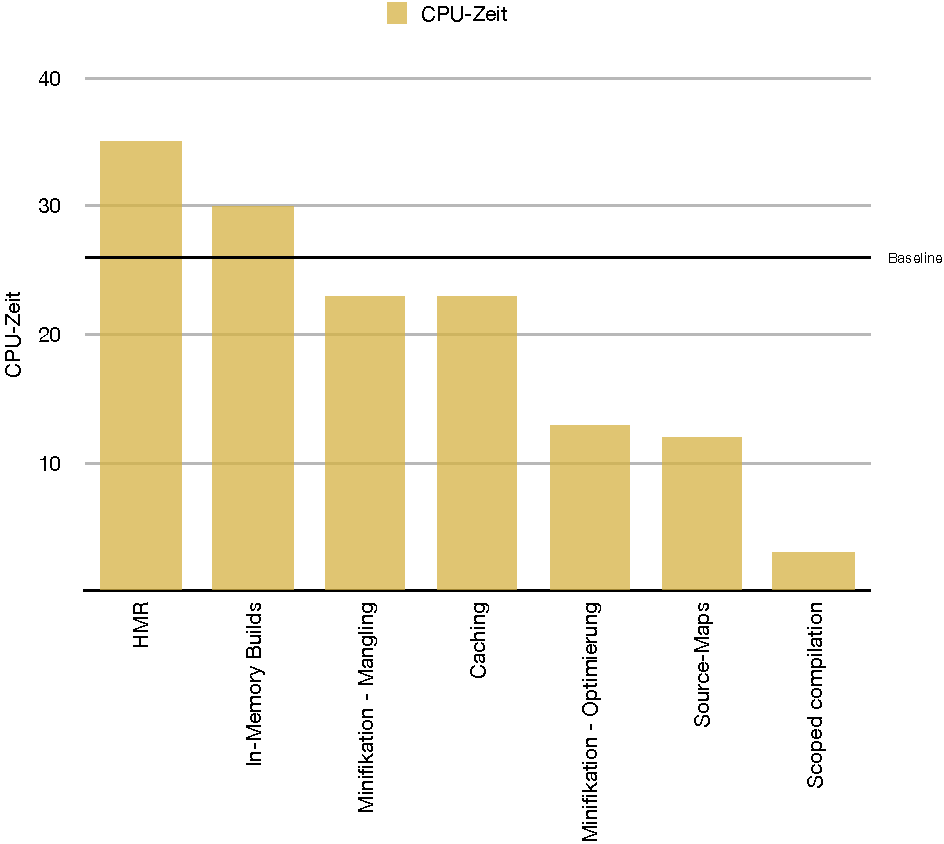
\includegraphics[width=\textwidth]{img/resultGraph}
            \caption{Vergleich aller Optimierungen}
            \label{figure:resultGraph}
		\end{figure}

		
		\section{Beeinflussbarkeit der Builddauer}
			\paragraph{Minifikation} Um die Optimierungen der Minifikation bezüglich der Build-Zeit umzusetzen Bedarf es lediglich einer kleinen Anpassung an der Konfiguration mit nur marginaler Auswirkung auf das Ergebnis. Allerdings stellt sich hierbei die Frage, ob Minifikation für Entwicklungs-Builds überhaupt notwendig ist oder komplett deaktiviert werden könnte. 
			\paragraph{Scoped compilation} Scoped compilation der Abhängigkeiten ist sehr einfach umzusetzen, indem man diese in einem extra Build mithilfe einer zweiten Build-Konfiguration separat baut. Ist das Projekt bereits in mehrere Module aufgeteilt, so kann man diese ebenfalls mit in einen eigenen Build übertragen und die Build-Zeit auf ein Minimum reduzieren. Entsprechend ist eine Modularisierung des Projektes von Beginn an anzustreben um Scoped compilation im vollen Potenzial nutzen zu können.
			\paragraph{Caching} Bei größeren Projekten mit vielen Dateien, welche nicht häufig angepasst werden, aber auch nicht in ein eigenes Modul ausgelagert werden können bietet sich Caching an. Wie im vorhergehenden Abschnitt beschrieben kommt Caching jedoch mit einem gewissen Overhead, welcher besonders bei In-Memory-Builds sichtbar wird. Dabei hängt es von der Größe des Projektes und der Geschwindigkeit sowie der Zugriffszeit der Festplatte ab, wann sich Caching auf der Festplatte lohnt.
			\paragraph{Source maps} Ob Source-Maps optimiert werden können hängt von dem Projekt ab. Wenn ein Entwickler diese häufig nutzt um Code zu debuggen und dies auf einer Zeilen-Basis tut, so ist es nicht von Vorteil diese zu deaktivieren bzw. ihren Scope zu vergrößern. Werden diese jedoch in der Entwicklung nur kaum oder gar nicht genutzt, so kann der sehr signifikante Performance Vorteil von über $50 \%$ durch eine einfache Anpassung der Konfiguration genutzt werden.
			\paragraph{Inkrementeller In-Memory Build \& \Gls{hmr}} Besonders für UI-Development und Prototyping bieten sich In-Memory-Builds zusammen mit \Gls{hmr} an, da sie es ermöglichen einzelne Komponenten in einer laufenden Instanz auszutauschen. Dies kommt jedoch mit einem zusätzlichen Konfigurationsaufwand. In-Memory Builds sind einfach zu aktivieren, aber \Gls{hmr} setzt eine Unterstützung von dem entsprechenden Framework voraus. Nutzt man z. B. React wie in dem Beispielprojekt so kann dies durch eine zusätzliche Anpassung der Konfiguration aktiviert werden. Im Fall von z. B. Angular erfordert dies zusätzlich eine Modifikationen von den Komponenten\cite{frameworks:angular-hmr}. Kurzum hängt der Funktionsumfang und die Komplexität der Integration von den genutzten Frameworks und dessen Support für \Gls{hmr} ab.\\
			
			Insgesamt sind viele der Optimierungen wie Minifikation, Scoped compilation und Caching durch minimale Anpassungen der Konfigurationsdatei einsetzbar. Optimierungen wie modulbasierte Source-Maps oder \Gls{hmr} hingehen sind von dem Projekt, dessen Aufbau, der genutzten Frameworks und dem Workflow abhängig.\\
			Geht man von dem Beispielprojekt aus so können in einem einfachen Projekt durch simple Anpassungen Verbesserungen der Build-Dauer um einen Faktor von bis zu $10$ im Vergleich zu der Ausgangskonfiguration erreicht werden. Werden weiterführende Features wie \Gls{hmr} von den Frameworks unterstützt und zeilenbasierte Source-Maps nicht benötigt, so kann dies sogar auf einen Faktor von bis zu $24$ erhöht werden\footnote{Da die Build-Dauer in diesen Messungen nur sehr gering war können die tatsächliche Einsparungen bei realen Projekten abweichen.}.\\
			Diese Analyse beschränkt sich auf Webpack doch einige der Anpassungen wie z. B. die Minifikation\cite{frameworks:uglifyJS} werden durch externe Libraries umgesetzt. Die Konfigurationsanpassungen lassen sich stellenweise also auch auf andere \Glspl{bundler} anwenden.

		\section{Zusammenfassung}
			Abschließend kann man sagen, dass es beeinflussbare Faktoren in dem Buildprozess von \Glspl{bundler} gibt, die gemeinsam einen signifikanten Performance-Vorteil bieten und somit den Entwicklungsprozess beschleunigen. Es wurde insgesamt eine Beschleunigung des Buildvorgangs um den Faktor $26$ erreicht und somit die Dauer auf knapp eine Sekunde reduziert, was nur ein Bruchteil der durchschnittlichen Aufmerksamkeitsspanne eines Menschen ausmacht. Somit kann verhindert werden, dass Software-Entwickler während des Buildprozess ihren Fokus verlieren und sich anderen Dingen zuwenden. Außerdem liegt der Wert weit unter dem Eingangs beschriebenen Schwellwert und sehr nahe an dem absoluten Minimum. Weitere Optimierungen sind somit im Fall des Beispiel-Projekt nicht mehr von Relevanz, da eine Veränderung von unter einer Sekunde nur schwer wahrnehmbar.
			
    \pagebreak

    %%%%%%%%%%%%%%
    %% Appendix %%
    %%%%%%%%%%%%%%
    \chapter{Appendix}
	    \hspace{0pt}
    \vfill
    \subsection*{Eidesstattliche Erklärung}
        Hiermit erkläre ich an Eides statt, dass ich die vorliegende Arbeit ohne Hilfe Dritter und ohne Benutzung anderer als der angegebenen Hilfsmittel angefertigt habe. Die aus fremden Quellen direkt oder indirekt übernommenen Gedanken sind als solche kenntlich gemacht. Die Arbeit wurde bisher in gleicher oder ähnlicher Form weder von mir noch von jemand anderem als Prüfungsleistung vorgelegt.
        \vspace{2cm}
        \SignatureAndDate{Unterschrift}
    \vfill
    \hspace{0pt}
    
    \clearpage
    
    \begin{lstlisting}[language=JavaScript,label={figure:baselineConfiguration},caption={Ausgangskonfiguration für Webpack 4 (webpack.config.js)}]
const path = require('path');
const webpack = require('webpack');
const HtmlWebpackPlugin = require('html-webpack-plugin');
const UglifyJsPlugin = require('uglifyjs-webpack-plugin');
const SpeedMeasurePlugin = require("speed-measure-webpack-plugin");
const smp = new SpeedMeasurePlugin({ outputFormat: 'human' });

module.exports = smp.wrap({
    mode: 'development',
    entry: './src/index.jsx',
    devtool: 'source-map',
    devServer: { contentBase: './dist' },
    output: {
        path: path.resolve(__dirname, 'dist'),
        filename: 'webpack-project.bundle.js'
    },
    module: {
        rules: [
            {
                test: /\.(js|jsx)$/,
                enforce: 'pre',
                use: [
                    {
                        options: {
                            eslintPath: require.resolve('eslint'),
                        },
                        loader: require.resolve('eslint-loader'),
                    },
                ],
                include: path.resolve(__dirname, 'src'),
            },
            {
                oneOf: [
                    {
                        test: [/\.bmp$/, /\.gif$/, /\.jpe?g$/, /\.png$/],
                        loader: require.resolve('url-loader'),
                        options: {
                            limit: 10000,
                            name: 'static/media/[name].[hash:8].[ext]',
                        },
                    },
                    {
                        test: /\.css$/,
                        use: [
                            'style-loader',
                            { loader: 'css-loader', options: { importLoaders: 1 } },
                            'postcss-loader'
                        ]
                    },
                    {
                        test: /\.(js|jsx)$/,
                        exclude: /(node_modules|bower_components)/,
                        use: {
                            loader: 'babel-loader',
                            options: {
                                compact: true,
                                cacheDirectory: true,
                                plugins: ['transform-class-properties'],
                                presets: ['env', 'react']
                            }
                        }
                    },
                    {
                        loader: require.resolve('file-loader'),
                        exclude: [/\.(js|jsx|mjs)$/, /\.html$/, /\.json$/],
                        options: {
                            name: 'static/media/[name].[hash:8].[ext]',
                        },
                    },
                ]
            }
        ]
    },
    optimization: {
        splitChunks: {
            chunks: 'all'
        }
    },
    plugins: [
        new HtmlWebpackPlugin({
            inject: true,
            template: 'src/index.html',
            minify: {
                removeComments: true,
                collapseWhitespace: true,
                removeRedundantAttributes: true,
                useShortDoctype: true,
                removeEmptyAttributes: true,
                removeStyleLinkTypeAttributes: true,
                keepClosingSlash: true,
                minifyJS: true,
                minifyCSS: true,
                minifyURLs: true,
            },
        }),
        new UglifyJsPlugin({
            uglifyOptions: {}
        }),
    ]
});
	\end{lstlisting}
	\pagebreak
	\begin{lstlisting}[language=JavaScript,caption={Scoped compilation Konfigurationsdatei (webpack.vendor.config.js)},label={vendorConfig}]
const path = require('path');
const webpack = require('webpack');

const outputPath = path.join(process.cwd(), 'dist');

module.exports = {
    context: process.cwd(),
    entry: {
        ReactStuff:[
            'react',
            'react-dom',
            '@material-ui/core',
            '@material-ui/icons',
            'victory',
            'prop-types'
        ]
    },

    output: {
        filename: '[name].dll.js',
        path: outputPath,
        library: '[name]',
    },

    plugins: [
        new webpack.DllPlugin({
            name: '[name]',
            path: path.join(outputPath, '[name].json')
        })
    ]
};
		        	\end{lstlisting}

    \glsaddall
    \printglossary
    \printglossary[type=\acronymtype]


    \nocite{*}
    \bibliography{main.bib}

\end{document}
